\documentclass{article}

% if you need to pass options to natbib, use, e.g.:
%     \PassOptionsToPackage{numbers, compress}{natbib}
% before loading neurips_2018

% ready for submission
% \usepackage{neurips_2018}

% to compile a preprint version, e.g., for submission to arXiv, add add the
% [preprint] option:
%     \usepackage[preprint]{neurips_2018}

% to compile a camera-ready version, add the [final] option, e.g.:
     \usepackage[final]{nips_2018}

% to avoid loading the natbib package, add option nonatbib:
%     \usepackage[nonatbib]{neurips_2018}

\usepackage[utf8]{inputenc} % allow utf-8 input
\usepackage[T1]{fontenc}    % use 8-bit T1 fonts
\usepackage{hyperref}       % hyperlinks
\usepackage{url}            % simple URL typesetting
\usepackage{booktabs}       % professional-quality tables
\usepackage{amsfonts}       % blackboard math symbols
\usepackage{nicefrac}       % compact symbols for 1/2, etc.
\usepackage{microtype}      % microtypography
\usepackage{amsmath}


\usepackage{graphicx}

\title{CECS 551 Project}

% The \author macro works with any number of authors. There are two commands
% used to separate the names and addresses of multiple authors: \And and \AND.
%
% Using \And between authors leaves it to LaTeX to determine where to break the
% lines. Using \AND forces a line break at that point. So, if LaTeX puts 3 of 4
% authors names on the first line, and the last on the second line, try using
% \AND instead of \And before the third author name.

\author{%
  Jared R.~Coleman\\
  Computer Engineering and Computer Science\\
  California State University, Long Beach\\
  Long Beach, CA 90802 \\
  \texttt{jared.coleman@student.csulb.edu} \\
  \And 
  Taina G.D.~Coleman\\
  Computer Engineering and Computer Science\\
  California State University, Long Beach\\
  Long Beach, CA 90802 \\
  \texttt{taina.coleman@student.csulb.edu} \\
  \And 
  Ian M. ~Schenck\\
  Computer Engineering and Computer Science\\
  California State University, Long Beach\\
  Long Beach, CA 90802 \\
  \texttt{ian.schenck@student.csulb.edu} \\
}

\begin{document}

\maketitle

\begin{abstract}
   Since its introduction in 2014, the Generative Adverserial Network (GAN) has been adapted and improved upon at Machine Learning conferences all over the world. In this short survey, we discuss the fundamentals of GAN and one of its successors, the Wasserstein GAN (WGAN).
\end{abstract}


\section{Introduction} 
The goal of any generative model is to learn a probability distribution from data. Given a set of observed data $X$, we wish to recover the probability distribution $P_r$ that it was drawn from. If we were able to find $P_r$ exactly, that would mean we could draw unlimited samples from the same distribution that generated $X$. For example, imagine $X$ is a set of images of bedrooms. If we could find the real probability distribution these images came from, we would be able to generate an image of a bedroom that doesn't exist in $X$. 


In practice, we want to find $argmin_\theta(d(P, P_\theta))$, where $d$ is some measure of distance (divergence) between probability distributions. If we were to find $P_\theta=P_r$, then drawing a sample from $P_\theta$ would be equivalent to drawing a sample from $P$. In practice, we hope to find a sufficiently close $P_\theta$ so that drawing a sample from $P_\theta$ \textit{appears} equivalent to drawing a sample from $P_r$.

There are many approaches to generative modeling, such as PixelRNN~\cite{Oord2016}, PixelCNN~\cite{Oord2016a}, and Variational Autoencoders (VAE)~\cite{Pu2016}. In this paper however, we will focus on the Generative Adversarial Network~\cite{Goodfellow2017} and one of its most successful successors, the Wasserstein Generative Adversarial Network~\cite{Arjovsky2017}.

\section{Generative Adversarial Networks (GAN)}

The GAN approach to generative modeling is unlike traditional approaches (PixelRNN, PixelCNN, VAE, etc.) in that its goal is not to find $P_\theta$. Rather, the goal is to find a function $G$ such that $G(z) \sim P_\theta, z \sim P_z~$ where $P_z$ is a \textit{previously known} probability distribution. In other words, GANs try to find a function that \textit{transforms} samples from a known distribution $P_z$ into samples from the target distribution $P_\theta$. We never actually find $P_\theta$, but that doesn't really matter since we are still able to draw samples from it. 

In the GAN architecture, two neural networks, a generator ($G$) and a discriminator ($D$) compete against each other (Figure \ref{fig:gan}). A common analogy for their relationship is that of a banker and a counterfeiter. The banker's goal is to discriminate between real and fake money while the counterfeiter's goal is to trick the banker into classifying his fake money as real. By participating in this game, the banker gets better at identifying fake money, and the counterfeiter gets better at manufacturing realistic fake money. In GANs, $G$ and $D$ play a similar game with each other until the samples generated by $G$ are so realistic enough that $D$ is forced to guess (with a 50\% chance of being correct) whether or not the sample is authentic. This can be formalized as a min-max game:

\begin{center}
	$\underset{G}{min}~\underset{D}{max}~\mathbb{E}_{x \sim P_r}~log~D(x) + \mathbb{E}_{z \sim P_z}~log~D(1-G(z))$
\end{center}

\begin{figure}[h!]
	\centering
	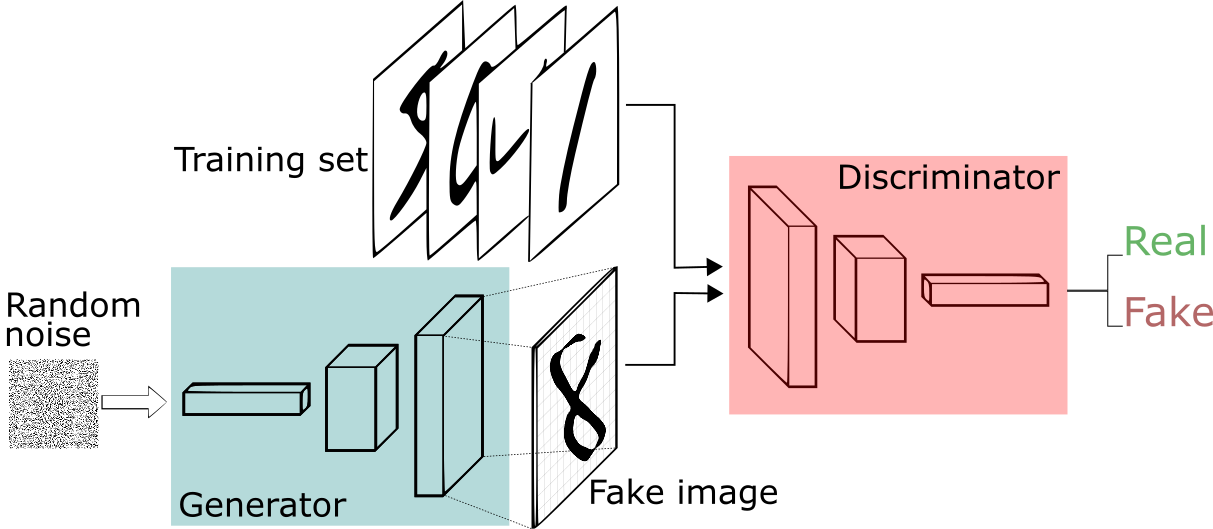
\includegraphics[width=\linewidth]{media/gan.png}
	\caption{Gan Architecture.  \textbf{https://medium.freecodecamp.org/an-intuitive-introduction-to-generative-adversarial-networks-gans-7a2264a81394}}
	\label{fig:gan}
\end{figure}

As an implementation detail, on the generator side, minimizing $-log~D(G(z))$ (or maximizing $log~D(G(z))$) is better than minimizing $log~D(1-G(z))$ since it's gradients are better for initial samples generated by $G$.

So for the discriminator, we want to maximize:

\begin{center}
	$\mathbb{E}_{x \sim P_r}~log~D(x) + \mathbb{E}_{z \sim P_z} log D(1-G(z))$
\end{center}

and for the generator, we want to maximize:

\begin{center}
	$\mathbb{E}_{z \sim P_z}~log~D(1-G(z))$
\end{center}

Since $D$ and $G$ are neural networks, we can maximize them with using Stochastic Gradient Descent. 

\section{Wasserstein GAN}

As mentioned in the past section, the training for GANs is usually very slow and unstable, so the Wasserstein Adversarial Network - WGAN was introduced as an improvement in order to make training less difficult. The layout of the WGAN is different than the regular GAN. Now we only have one neural network in the model, the Generator, and a system that the author of the WGAN paper \cite{Arjovsky2017} calls the critic. Instead of using another NN to classify the data as real or fake, WGAN uses the critic to find the distance function in between a real data probability distribution and a fake one, and then uses this function to calculate the loss, and finally update the weights to start a new iteration.

When training GAN models the goal is to find a distribution $P_{\theta}$ that is the most similar to a real distribution $P_{r}$, where $\theta$ is the parameters. There are two approaches to perform this task:
1. Define a parametric family of densities $P_{\theta}$, which is as a differentiable function $P_{\theta} >= 0$ and integral ($P_{\theta}$(x) dx) = 1, where x is a real data sample. Try to directly learn $P_{theta}$ by optimizing it through maximum likelihood estimation (MLE).
2. Define a variable Z with an existent distribution $p(z)$ and pass it through the Generator, $g_{\theta}$, that will generate samples that follow the distribution $P_{theta}$. By updating $\theta$ the $P_{theta}$ can be modified to get more similar to $P_{r}$.

The first approach usually runs into problems since trying to maximize MLE:
\textbf{insert MLE equation here}

Is the same as trying to minimize KL divergence.
(maybe insert proof here or just the KL equation).

In KL divergence if Q(x) = 0, which in this case is $P_{theta}$, for a $x$ where $P_{r}(x) > 0$, the result goes to +infinity. This makes improbable for $P_{r}$ to fall within that support in low dimensional manifolds, which means that if one point of $P_{theta}$ lays outside of the support, KL will not be defined. In order to try to remediate this problem, a noise term called the Gaussian noise, with a large enough bandwidth to cover all the examples, is added to the distribution $P_{theta}$. Although by taking this maneuver, error is being added to the system resulting in poor quality images. Also, even if a density $P_{theta}$ is learned, it could be computationally expensive to sample from it REF (read-through).

The latter approach has two big advantages: it can represent distributions in a low dimension manifold, and unlike the densities, it is easier to generate samples of the distribution. This specific approach is the focus of the main reference for this survey. To get to the goal of finding a distribution $P_{theta}$ as close to $P_{r}$ as possible, the parameter $\theta$ needs to be optimized, in which the mapping $\theta -> P_{theta}$ should be continuous, since the objective is when a sequence of parameters converge to $\theta$, the distribution correspondent to those parameters converges to $P_{theta}$. To measure the similarity, or distance in between the distributions in order to keep fine tuning $\theta$, the paper goes on to present various metrics that are commonly used. 



\section{Graph Convolutional Networks}
\subsection{Background}
The success of deep learning paradigms such as convolutional neural networks (CNN) with Euclidean data such as images, text and video has led to research on how non-Euclidean data such as graphs can be effectively analyzed through deep learning. In a standard CNN, convolutions are relatively simple to compute, as input sizes are always uniform. Graphs make this more complicated, as they can have different numbers of unordered nodes, each with different numbers of neighbors~\cite{Wu2019}. The first major research on graph convolutional networks (GCN) is based on spectral graph theory~\cite{Bruna2013}, which is the analysis the properties and the structure of a graph from its spectrum, or set of eigenvalues and eigenvectors. In this overview we will mostly discuss Kipf et al.'s research on semi-supervised classifications using GCNs~\cite{Kipf2016}, which is based on a first-order approximation of the localized spectral filters on graphs developed in previous research on GCNs~\cite{Bruna2013}. 

GCNs based on spectral graph theory look at spectral convolutions as removing noise from a graph signal $x \in \mathbb{R}^n$ with a filter $g_\theta$,
\stepcounter{equation}
\setcounter{equation}{0}
\begin{equation}
\label{spectral_prop}
g_\theta \star x = Ug_\theta U^Tx
\end{equation}
$g_\theta$ is understood as a function of eigenvalues of the normalized graph laplacian, $L = I_N - D^{-\frac{1}{2}}AD^{-\frac{1}{2}}$ where $A$ is the graph's adjacency matrix and $D$ is a diagonal matrix of node degrees, $D_{ii} = \sum_{j} (A_{i,j})$. $L$ is a real symmetric posiive semidefinite, so it can be factored to $L = U\Lambda U^T$, where $U$ is a matrix of eigenvectors ordered by eigenvalues, and $\Lambda$ is is the diagonal matrix of eigenvalues. Multiplication with $U$ is $\mathcal{O}(N^2) $ and finding the eigenvectors and eigenvalues of $L$ can grow very expensive for large graphs. To reduce the computational cost of GCNs, a truncated expansion of Chebyshev polynomials could be used to approximate $g_\theta (\Lambda)$~\cite{Defferrard2016}.
Chebyshev polynomials are defined recursively as $T_k(x) = 2xT_{k-1}(x) - T_{k-2}(x)$ with $T_0(x) = 1$ and $T_1(x) = x$~\cite{Hammond2011}.
\begin{equation}
\label{cheby_prop}
g_{\theta'} \star x \approx \sum\limits_{k=0}^{K} \theta'_k T_k (\tilde{L})x
\end{equation}
$T_k(\tilde{L})$ is the Chebyshev polynomial of order $k$, and $\tilde{L} = \frac{2}{\lambda_{max}} L - I_n$. This approximation avoids any multiplication with $U$, significantly reducing the computation time. Because $T_k(\tilde{L})$ is only dependent on the neighbors at most $K$ steps away, whereas the entire graph is used in Equation $(\ref{spectral_prop})$.

The propagation rule proposed in Kipf et al. further approximates Equation 
$(\ref{cheby_prop})$ by assuming $K = 1$, which reduces the computational cost even more and reduces overfitting on graphs with wide node degree distributions~\cite{Kipf2016}. Furthermore, they set $\lambda_{max} = 2$, which reduces $\tilde{L} = \frac{2}{2}L - I_N = I_n - D^{-\frac{1}{2}}AD^{-\frac{1}{2}} - I_N = D^{-\frac{1}{2}}AD^{-\frac{1}{2}}$. These simplified values can be plugged in to Equation $(\ref{cheby_prop})$:
\begin{equation}
\label{reduce_k}
g_{\theta'} \star x \approx \sum\limits_{k=0}^{1} \theta'_k T_k (D^{-\frac{1}{2}}AD^{-\frac{1}{2}})x = \theta'_0 T_0(D^{-\frac{1}{2}}AD^{-\frac{1}{2}})x + \theta'_1 T_1(D^{-\frac{1}{2}}AD^{-\frac{1}{2}})x 
\end{equation}
Recalling the recursive definition of Chebyshev polynomials described above, this simplifies to:
\begin{equation}
\label{simplified_1stcheby}
g_{\theta'} \star x \approx \theta'_0x + \theta'_1 D^{-\frac{1}{2}}AD^{-\frac{1}{2}}x 
\end{equation}
To reduce overfitting and minimize operations per layer, they only used a single parameter $\theta = \theta'_0 = -\theta'_1$, allowing the equation to be factored in this form:
\begin{equation}
\label{single_param}
g_\theta \approx \theta(I_N + D^{-\frac{1}{2}}AD^{-\frac{1}{2}})x
\end{equation}
One issue with this approximation is $\lambda_{max} = 2$, meaning the eigenvalue range is $[0,2]$, which they found could cause numerical instability and exploding/vanish gradients in the GCN~\cite{Kipf2016}. They added self connections to the adjacency matrix, $\tilde{A} = A + I_N$, and used the diagonal matrix of the node degrees of $\tilde{A}$, replacing $I_N + D^{-\frac{1}{2}}AD^{-\frac{1}{2}}$ with $\hat{A} = \tilde{D}^{-\frac{1}{2}}\tilde{A}\tilde{D}^{-\frac{1}{2}}$. These additions bring us to the layer-wise propagation rule:
\begin{equation}
\label{prop_rule}
H^{(l+1)} = \sigma(\hat{A}H^{(l)}W^{(l)})
\end{equation}
$H^{(l)} \in \mathbb{R}^{N x C}$ is the input signal, where $H^{(0)} = X$, and $W^{(l)} \in \mathbb{R}^{C x F}$ is the filter parameter matrix for the current layer, $\sigma(\cdot)$ is an activation function, and $H^{(l+1)} \in \mathbb{R}^{N x F}$ is the convolved signal matrix~\cite{Kipf2016}. The renormalized adjancency matrix $\hat{A}$ can be represented as a sparse matrix, so multiplying $\hat{A}$ by $H^{(l)}$ only has a complexity of $\mathcal{O}(|\mathcal{E}|)$, giving the entire operation a complexity of $\mathcal{O}(|\mathcal{E}|FC)$.  This new graph convolution is localized in space, so each row of the output $Z$ contains a latent representation of each node of input $X$ as well as its neighbors, with values from $\hat{A}$ determining how much weight each neighbor is given in the latent representation.

\subsection{Model Architecture and Experiments}
With Equation \ref{prop_rule}, they build a deep learning model for semi-supervised node classification, where the goal is to classify all nodes in a graph where only a few have labels. They made a forward model for a two layer network using the propagation rule in Equation \ref{prop_rule}:
\begin{equation}
\label{forward_model}
Z = f(X, A) = softmax(\hat{A} ReLU(\hat{A}XW^{(0)})W^{(1)})
\end{equation}
In this model, $W^{(0)} \in \mathbb{R}^{C x H}$ and $W^{(1)} \in \mathbb{R}^{H x F}$, $H$ being number of hidden features, and $F$ being the number of output features.
In a supervised learning network, we could then calculate cross-entropy loss for all training examples, but in this semi-supervised learning network, only a few examples have labels, so they evaluate loss by calculating cross-entropy error for each labeled example. Then $W^{(0)}$ and $W^{(1)}$ are trained via gradient descent.
To experiment with this model, they trained it on three citation networks, with 20 labeled examples per class, a dataset extracted from a knowledge graph with only one labeled example per class, and random, featureless graphs with dummy labels. For the citation networks, they trained each model for maximum $200$ epochs, using a dropout rate of $0.5$ prior to both convolutions, $16$ units in the hidden layer, the Adam optimizer, a learning rate of $0.01$, weight decay of $0.0005$, Xavier weight initialization, and an early stop tolerance of 10 epochs of stagnant validation loss before ending training. 

After training the models, they compared mean classification accuracy of 100 runs with six other models, and found that their model had higher accuracy than the rest for each dataset. After comparing to other models, they compared the classification accuracy of the final propagation model from Equation $(prop_rule)$ against the others discussed in the paper: the Chebyshev filter from Equation $(\ref{cheby_prop})$, the $1^{st}$-order approximation from Equation $(\ref{reduce_k}$, the single parameter version from Equation $(\ref{single_param})$, and two others: a multilayer perceptron $X\Theta$ and a single order approximation without $I_N$: 
$D^{-\frac{1}{2}}AD^{-\frac{1}{2}}X\Theta $. Again, their model had superior accuracy compared to all the rest.

Finally, they compared their two-model layer with models from one to ten layers deep, along with a variant that uses residual connections between layers by adds the hidden layer $H^{(l)}$ to the propagation model in Equation $\ref{prop_rule}$, which allows for training with deeper models. They found that for the citation networks, 2 or 3 layer models gave the best results, with or without the previous layer's connections added. At deeper layers, the  

\section{Conclusion \& Future Work}

\bibliographystyle{plain}
\bibliography{references}

\end{document}

